\section{Marco tecnológico}

\noindent El procesamiento de información en diversos formatos es una tarea cada vez más importante. En un mundo cada vez más digital, es necesario poder procesar datos en una amplia variedad de formatos, desde lenguajes de programación hasta formatos de documentos y datos estructurados.

En este contexto, los generadores de reconocedores gramaticales, como JavaCC, ofrecen una solución muy prometedora. Estos generadores permiten crear analizadores léxicos y sintácticos a partir de una gramática definida por el usuario. Esto los hace muy versátiles y adaptables a una amplia variedad de gramáticas.

La aplicación de JavaCC en la asignatura Procesamiento de la Información en Aplicaciones Telemáticas (PIAT) es una idea muy acertada, ya que PIAT es una asignatura que se centra en el procesamiento de información en diversos formatos. Además, el uso de JavaCC podría proporcionar a los estudiantes una herramienta muy valiosa para abordar las prácticas de la asignatura.

\subsection{Analizador Léxico (Lexer)}

\noindent En el contexto de los analizadores de compiladores, un \textbf{analizador léxico} (del griego \lstinline|lexis|, palabra) ---también conocido como \textit{lexer}--- es la \textbf{primera fase} del proceso de \textbf{compilación}. Como se ilustra en la \autoref{fig:analizadorlexico}, su función es analizar el código fuente de un fichero y producir una secuencia de tokens o componentes léxicos\cite{lexer}. Con esto conseguimos reconocer tokens ---se hablarán de ellos más adelante--, ya que el analizador léxico divide la sintaxis del programa en una serie de tokens ---palabras clave, identificadores, operadores...--- y es capaz de eliminar cualquier información no relevante para el análisis posterior, como espacios adicionales o comentarios. 

Adicionalmente, si encuentra tokens inválidos o mal formados, el analizador léxico tiene la capacidad de generar mensajes de error. En última instancia, el analizador léxico \textbf{se encarga de preparar la entrada para} el siguiente paso del proceso de compilación, que es \textbf{el análisis sintáctico}.

%GramáticaTokenManager es literalmente el analizador léxico
%SimpleCharStream se usa para leer los tokens. Usa por debajo clases como Reader


\begin{figure}[H]
	\centering
	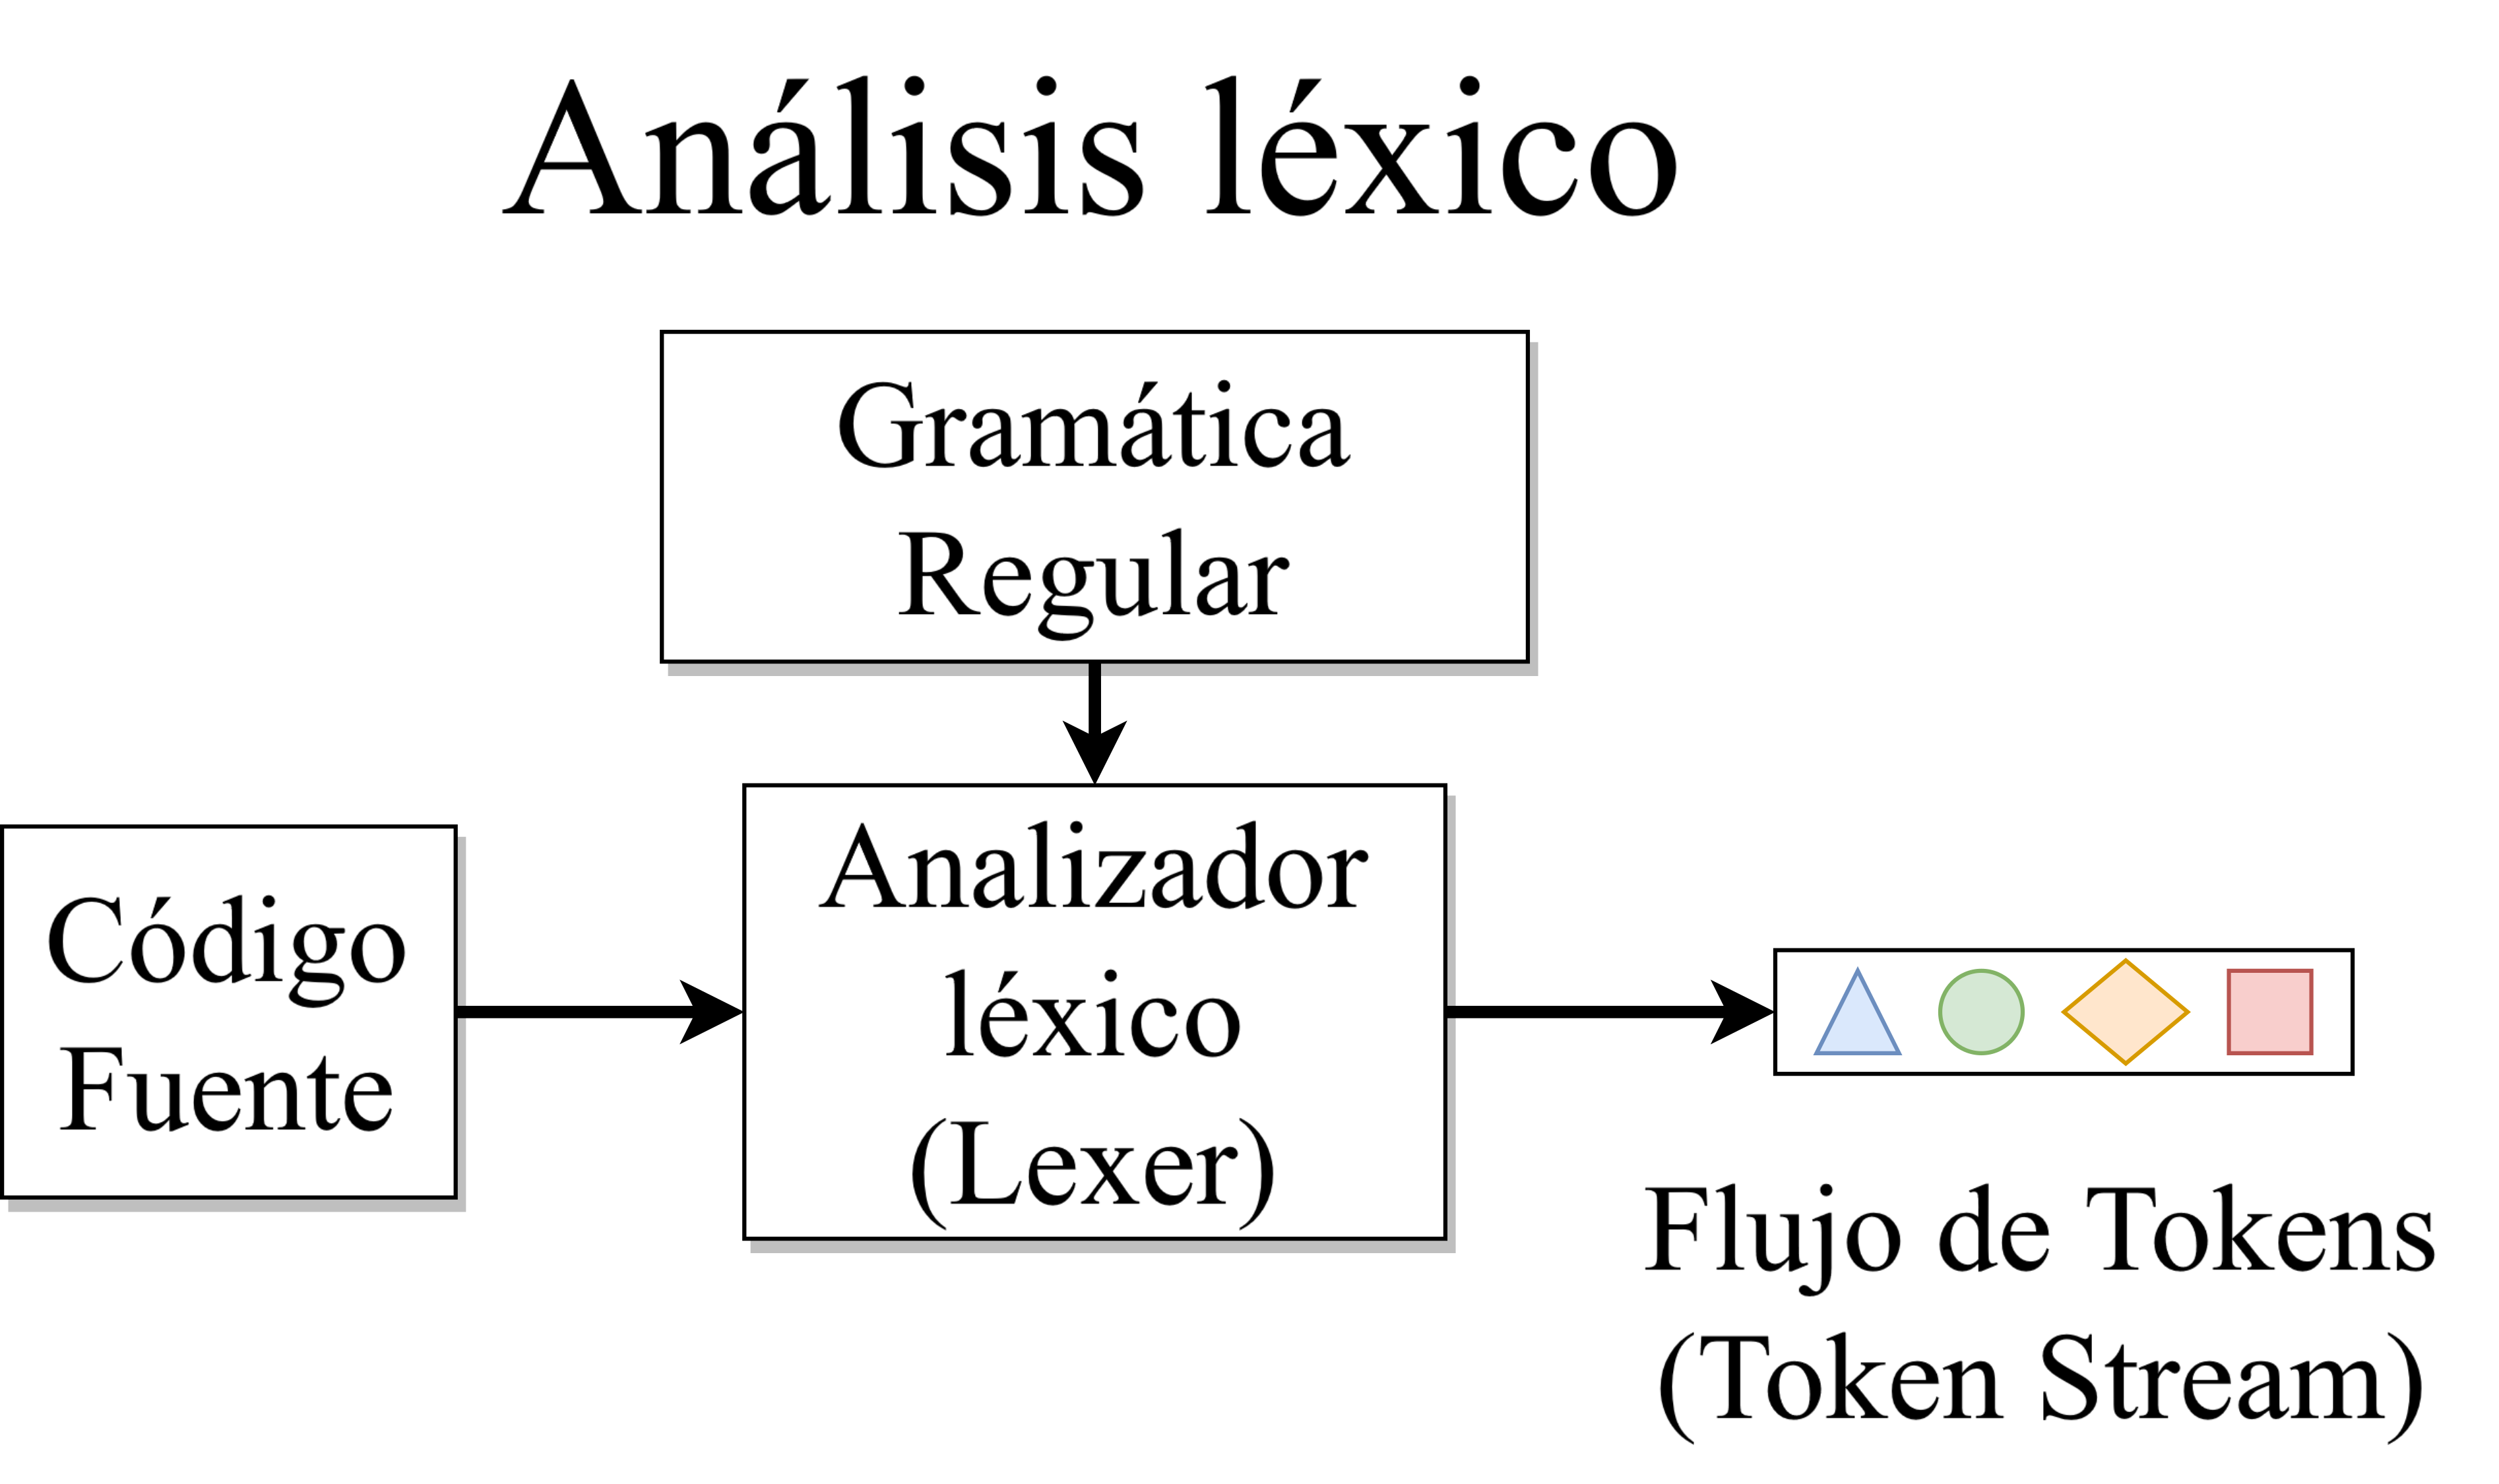
\includegraphics[width=0.8\textwidth]{imagenes/analizadorlexico.png}
	\caption{Funcionamiento del Analizador Léxico en JavaCC\cite{ytanalizadorlexico}}
	\label{fig:analizadorlexico}
\end{figure}

Supongamos que tenemos la siguiente frase: \lstinline|How Pleasant Is The Weather?| . Aquí podemos reconocer fácilmente que hay cinco palabras: “\textit{How}”, “\textit{Pleasant}”, “\textit{Is}”, “\textit{The}” y “\textit{Weather}.” Esto es natural para nosotros, ya que podemos identificar los separadores ---espacios en blanco--- y el símbolo de puntuación.

Ahora, consideremos una variante de la misma frase: \lstinline|HowPl easantIs Th ewe ather?|. Aquí es donde entra en juego el analizador léxico. Aunque también podemos leer esta versión, llevará más tiempo porque los separadores se colocan en lugares impares. No es algo que se entienda de inmediato.

El analizador léxico escanea el código fuente y reconoce los tokens incluso en situaciones más complejas como esta. En este caso, identificaría las palabras como tokens individuales, a pesar de la falta de espacios.

Se podría aplicar este concepto ilustrando otro ejemplo, más orientado a analizar archivos de código. Supongamos un fragmento de código en un lenguaje de programación ficticio como este:

\lstset{inputencoding=utf8/latin1}
\lstinputlisting{code/lexer.txt}

En este caso, el analizador léxico se encargaría de escanear este código fuente y dividirlo en tokens significativos. El analizador léxico reconocería las palabras clave como \lstinline|suma|, \lstinline|resta|, \lstinline|multiplicacion|, y \lstinline|division|. Además, también identificaría los operadores aritméticos como \lstinline|+|, \lstinline|-|,  \lstinline|*|, y  \lstinline|/|, así como números enteros como  \lstinline|10|,  \lstinline|20|,  \lstinline|30|,  \lstinline|15|,  \lstinline|5|, y \lstinline|6|. Por otra parte, el analizador léxico eliminaría cualquier espacio en blanco o comentario presente en el código. El resultado sería una secuencia de tokens --- o \textit{Flow Stream}--- como sigue:

\lstset{inputencoding=utf8/latin1}
\lstinputlisting{code/lexerresultado.txt}


\phantom{text}

\noindent \textbf{¿Qué es un token?}

\phantom{text}


\noindent Un token es una unidad léxica o componente básico del código fuente de un programa. Se trata de una cadena de caracteres con un significado específico asignado. Está estructurado como un par que consta de un nombre de token y un valor de token opcional. El nombre del token representa una categoría o tipo de unidad léxica, como palabras clave, identificadores, operadores, entre otros\cite{token}.

En el ejemplo de la sección anterior, el analizador léxico generaba una secuencia de tokens, en el que cada token tenía sus características propias, dependiendo de si eran identificadores, operadores o signos de puntuación, u otros ---se pueden especificar tokens que hagan referencias a comentarios dentro del código, o palabras reservadas del lenguaje, como \lstinline[keywordstyle=\color{black}]|if| o \lstinline[keywordstyle=\color{black}]|while|---. Estudiaremos más sobre los tokens y su funcionamiento en la sección \hyperref[sec:tokensenjavacc]{\textit{2.2.2. Tokens en JavaCC}}.


\subsection{Analizador Sintáctico (Parser)}
\noindent Un \textbf{analizador sintáctico} es una parte fundamental de un \textbf{compilador} o intérprete. Su función es verificar si un programa fuente ---escrito en un lenguaje de programación--- sigue las reglas gramaticales definidas para ese lenguaje\cite{analizadorsintactico}. En otras palabras, nos indica la disposición correcta de los elementos en el código fuente para que se convierta en un programa válido.

Comúnmente conocido como \textit{parser}, el analizador sintáctico verifica la \textbf{estructura} del programa fuente. Este hace uso de una gramática ---generalmente una gramática libre de contexto--- para definir las reglas sintácticas del lenguaje. El objetivo del parser es reconocer la secuencia de \textit{tokens} ---unidades léxicas como palabras clave, identificadores, operadores--- y construir un \textbf{árbol sintáctico} que represente la estructura jerárquica del programa. El funcionamiento del parser en JavaCC se describe en la \autoref{fig:analizadorsintactico}. Si el archivo fuente es válido, el analizador sintáctico proporciona el árbol sintáctico correspondiente.

Además de todas las funciones mencionadas, si encuentra errores sintácticos, como paréntesis desequilibrados o expresiones mal formadas, el analizador sintáctico genera mensajes de error\cite{traductorescompiladoreseinterpretes}. De esta forma ayuda a los programadores a identificar y corregir problemas en el código fuente de una manera sencilla y muy efectiva. Otras funciones que los analizadores sintácticos pueden desempeñar son el acceder a la tabla de símbolos, ya que necesita información sobre variables, funciones y otros símbolos definidos en el programa; el chequeo de tipos, ya que a menudo se verifica la compatibilidad de tipos ---por ejemplo, si se está aplicando un operador a operandos compatibles---, y la generación de código intermedio, proporcionando así una representación más abstracta y simplificada del programa.

\begin{figure}[H]
	\centering
	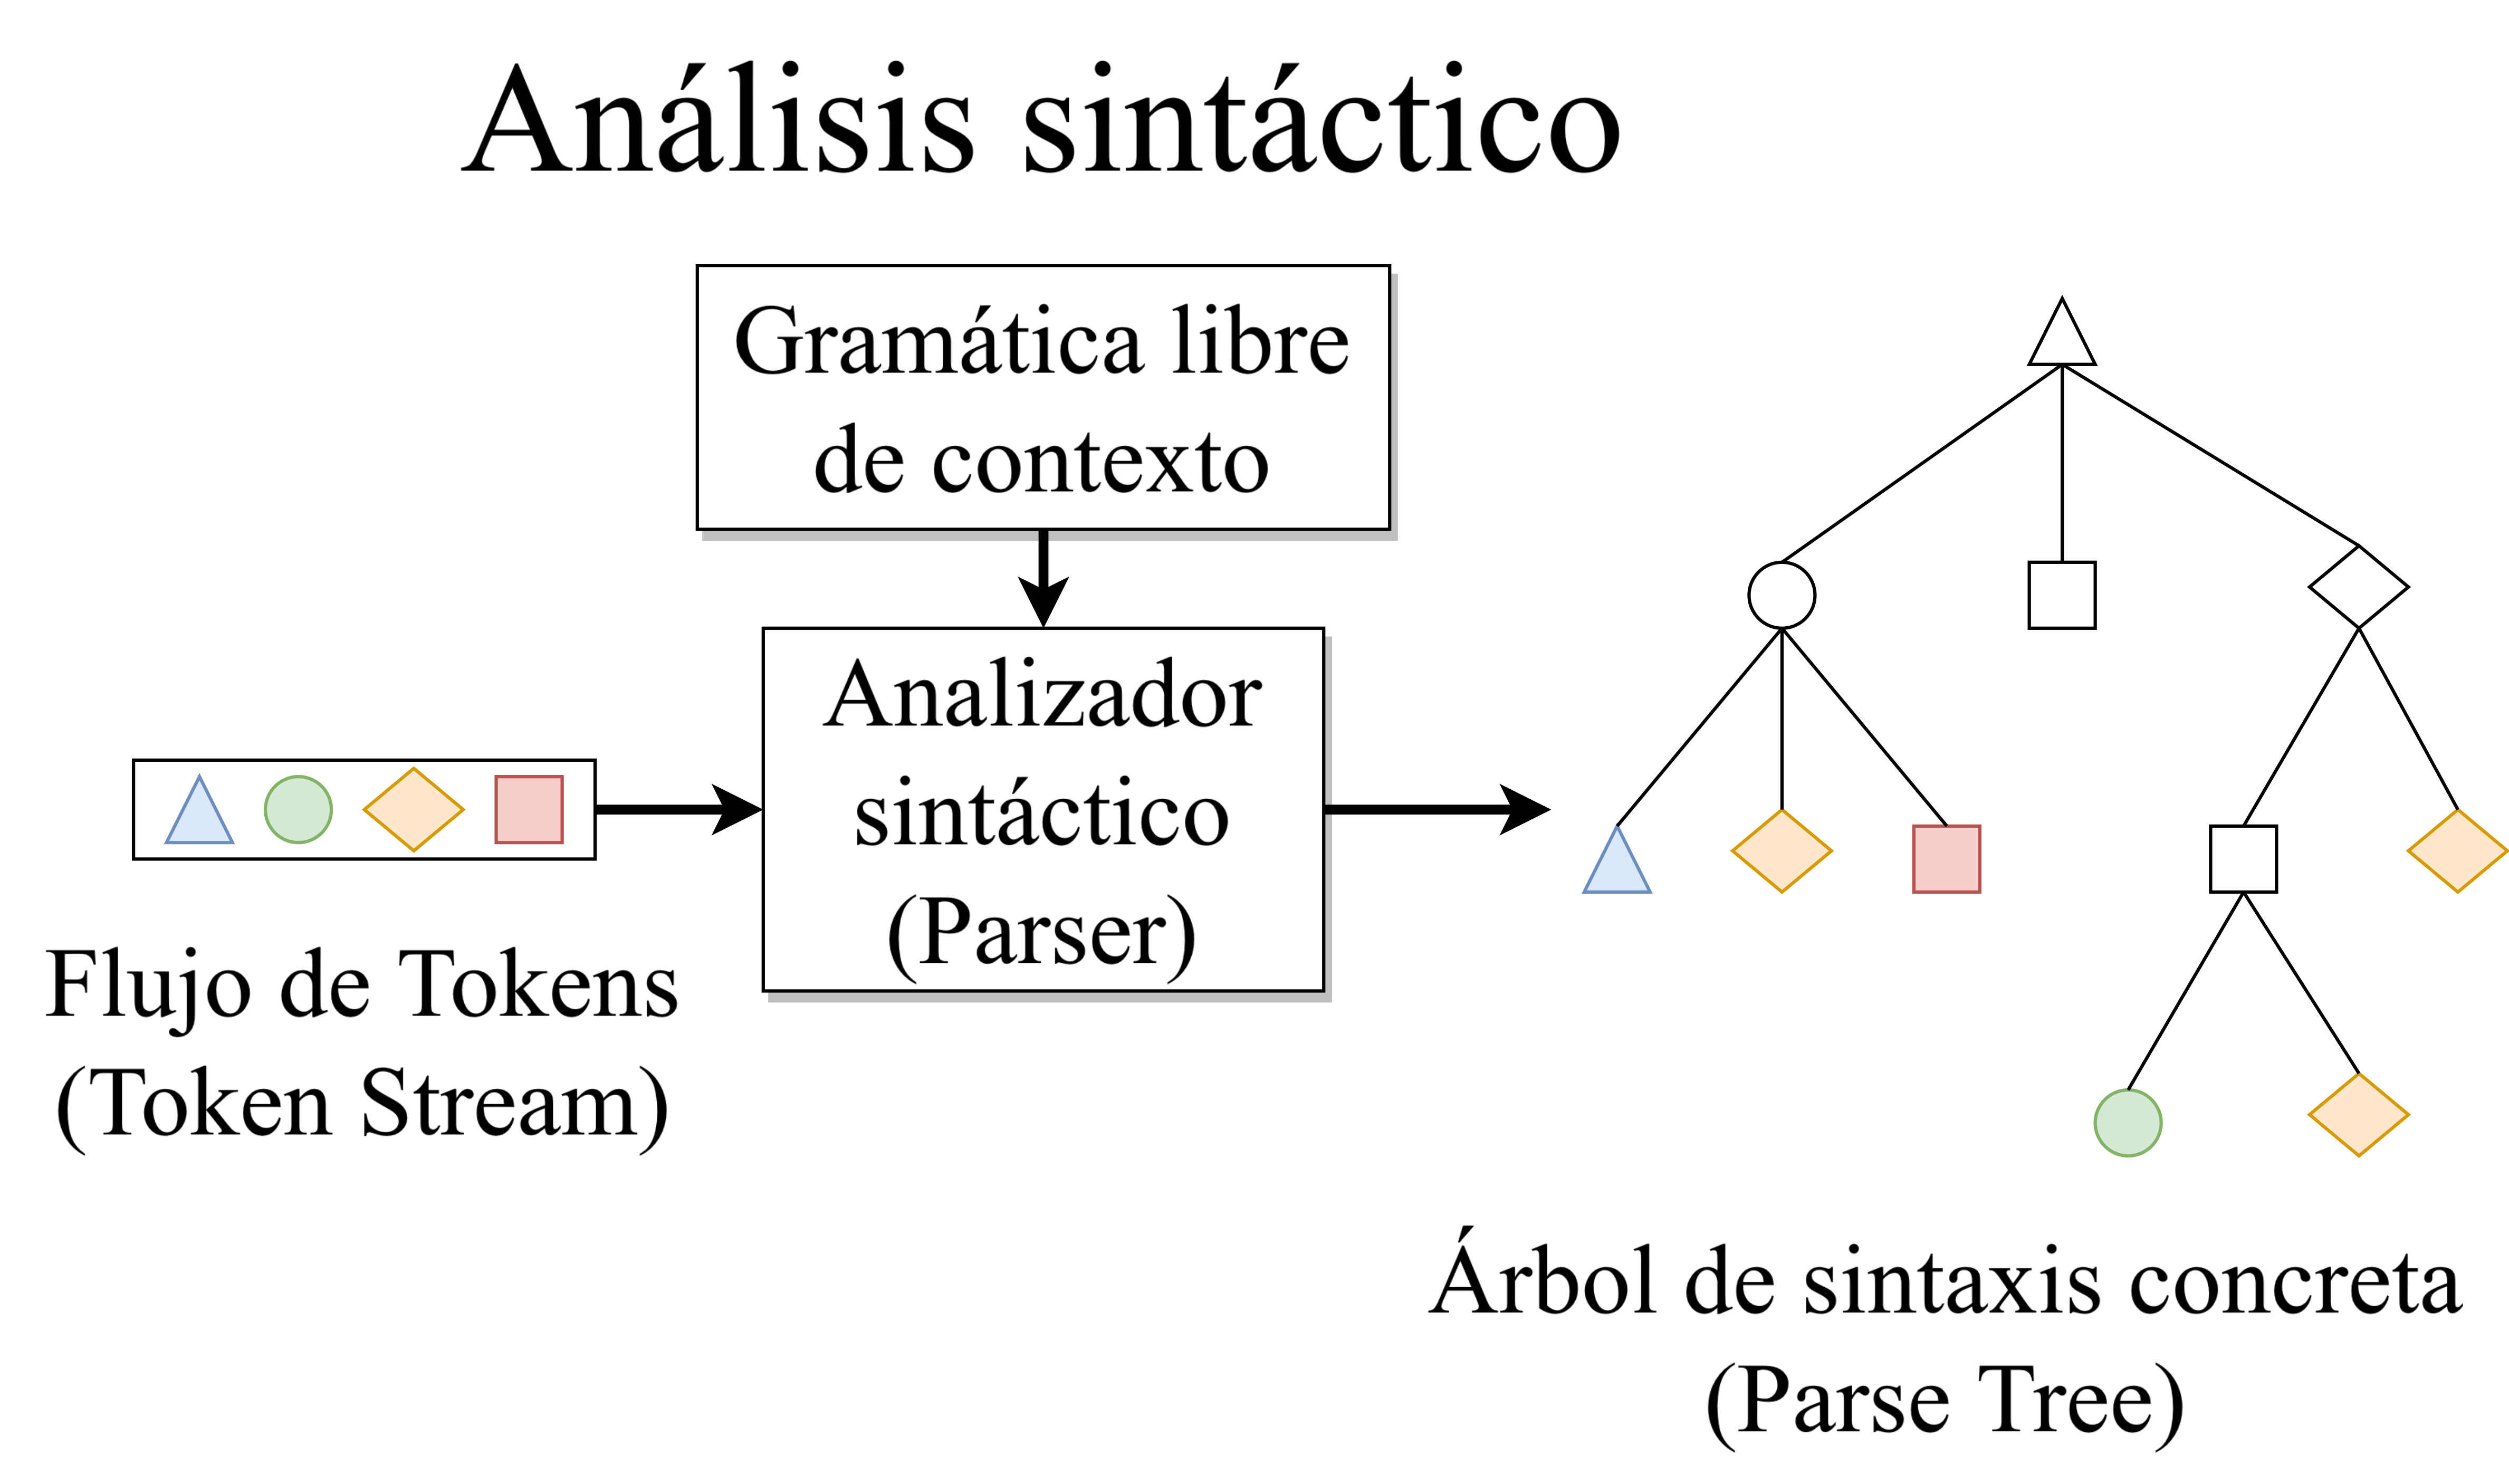
\includegraphics[width=\textwidth]{imagenes/analizadorsintactico.png}
	\caption{\label{fig:analizadorsintactico}Funcionamiento del Analizador Sintáctico en JavaCC\cite{ytanalizadorsintactico}}
\end{figure}

% \subsection{Recursividad}

% \noindent En el ámbito de los compiladores, la recursividad es una técnica que se utiliza para definir una estructura gramatical que se repite en sí misma.

% Esto permite resolver problemas complejos dividiéndolos en subproblemas más pequeños. Este proceso se repite hasta que se llega a subproblemas que son triviales de resolver.

% En JavaCC, la recursividad se utiliza para definir producciones gramaticales que pueden analizar expresiones complejas.

% \subsubsection{Recursividad a derechas (LR)}
% \noindent En la recursividad a derechas, la llamada recursiva se realiza al final de la definición de la estructura gramatical. Por ejemplo, la gramática para la expresión aritmética básica se puede definir recursivamente a la derecha de la siguiente manera:

% \lstset{inputencoding=utf8/latin1}
% \lstinputlisting{code/LR.jj}

% \subsubsection{Recursividad a izquierdas (LL)}

% \noindent En la recursividad a izquierdas, la llamada recursiva se realiza al principio de la definición de la estructura gramatical. Por ejemplo, la gramática para la expresión aritmética básica se puede definir recursivamente a la izquierda de la siguiente manera:

% \lstset{inputencoding=utf8/latin1}
% \lstinputlisting{code/LL.jj}



% Si considerásemos una producción recursiva a la izquierda, en caso de que la  condición fuera verdadera alguna vez, tendríamos una recursión infinita.
% JavaCC producirá un mensaje de error si tiene producciones recursivas a la izquierda.

\section{JavaCC}
\noindent En relación con lo anterior, aclaremos a qué hace referencia el concepto de JavaCC y los analizadores semánticos y sintácticos, y como se interrelacionan:
Java Compiler Compiler, comúnmente conocido como JavaCC, es una herramienta ampliamente utilizada para generar analizadores sintácticos en aplicaciones Java. Su función principal es transformar una especificación gramatical en un programa Java capaz de reconocer y analizar la sintaxis según la gramática proporcionada.
JavaCC se diferencia de otras herramientas similares al generar analizadores sintácticos de arriba hacia abajo ---descenso recursivo, o \textbf{(LL)?}--- en lugar de analizadores de abajo hacia arriba. Esta característica permite el uso de gramáticas más generales y facilita la depuración, además de permitir el análisis en cualquier elemento no terminal de la gramática y la transferencia de valores (atributos) en ambas direcciones en el árbol de análisis.

\subsection{Funciones principales de JavaCC}
% \noindent JavaCC ofrece una serie de características y funcionalidades clave que lo hacen destacar como un generador de analizadores sintácticos:
% \begin{itemize}
% 	\item Generación de analizadores sintácticos de arriba hacia abajo.
% 	\item Resolución de ambigüedades de cambio de turno localmente.
% 	\item Generación de analizadores 100\% Java puro.
% 	\item Especificaciones BNF extendidas.
% 	\item Integración de especificaciones léxicas y gramaticales en un solo archivo.
% 	\item Manejo de la entrada Unicode completa.
% 	\item Soporte para tokens no distinguibles entre mayúsculas y minúsculas.
% 	\item Herramientas adicionales como JJTree para construir árboles y JJDoc para generar documentación.
% 	\item Personalización a través de numerosas opciones.
% 	\item Informes de errores de alta calidad y mensajes de diagnóstico completos.
% \end{itemize}

% La estructura si sigue todo programa en JavaCC es el siguiente:

% \begin{figure}[H]
% 	\centering
% 	\includegraphics[width=\textwidth]{imagenes/estructuraprogramajavacc.png}
% 	\caption{\label{fig:estructuraprogramajavacc}Estructura de un programa en JavaCC \cite{estructuraprogramajavacc}}
% \end{figure}

% % \textbf{...DIAGRAMA CON ESTRUCTURA DE UN ANALIZADOR JAVACC...EXPLICAR QUE SOLO GENERAS UNA GRAMATICA, EXPLICAR LAS CLASES...AÑADIRLO EN UNA SUBSECCION...}

\noindent JavaCC se distingue como una herramienta potente para la generación de analizadores sintácticos gracias a un conjunto de características y funcionalidades clave. En primer lugar, su capacidad para generar analizadores sintácticos descendentes (\textit{top-down}) lo diferencia de otras herramientas y facilita la depuración, permitiendo un análisis más general de las estructuras gramaticales. Además, JavaCC destaca por su capacidad para resolver ambigüedades de cambio de turno de forma local, lo que simplifica el proceso de análisis.

Otro aspecto importante es que JavaCC genera analizadores escritos completamente en Java, lo que facilita su integración en proyectos Java y aprovecha las ventajas de este lenguaje. Además, JavaCC soporta especificaciones BNF extendidas, lo que permite definir gramáticas complejas con mayor flexibilidad.

A diferencia de otras herramientas, JavaCC integra las especificaciones léxicas y gramaticales en un único archivo, simplificando la gestión del código. También destaca su capacidad para manejar la entrada Unicode completa, lo que lo hace adecuado para proyectos internacionales.

JavaCC ofrece soporte para tokens que no distinguen entre mayúsculas y minúsculas, lo que puede ser útil en ciertos contextos. Además, se complementa con herramientas adicionales como JJTree para la construcción de árboles de análisis y JJDoc para generar documentación del código.

La personalización es otro punto fuerte de JavaCC, ya que ofrece numerosas opciones para adaptar su funcionamiento a las necesidades del proyecto. Finalmente, JavaCC proporciona informes de errores de alta calidad y mensajes de diagnóstico completos, lo que facilita la identificación y corrección de errores en la gramática.

\begin{figure}[H]
	\centering
	\includegraphics[width=\textwidth]{imagenes/estructuraprogramajavacc.png}
	\caption{\label{fig:estructuraprogramajavacc}Estructura de un programa en JavaCC \cite{estructuraprogramajavacc}}
\end{figure}

La creación de un programa con JavaCC implica una estructura específica que involucra diversos archivos y herramientas, como se puede observar en la \autoref{fig:estructuraprogramajavacc}. El proceso comienza con la definición de la gramática en un archivo con extensión ``.jj''. Este archivo contiene las reglas léxicas y sintácticas que definen el lenguaje a analizar.

JavaCC, actuando como un compilador, procesa este archivo ``.jj'' y genera un conjunto de archivos Java que conforman el analizador léxico y sintáctico. %Entre estos archivos se encuentran ``Gramática.java'', ``GramáticaConstants.java'' y ``GramáticaTokenManager.java''.% 
Estos archivos contienen las clases Java necesarias para realizar el análisis léxico y sintáctico del lenguaje definido en la gramática.

Para utilizar el analizador generado, se necesita un compilador Java que compile estos archivos y genere los correspondientes archivos ``.class''. Estos archivos ``.class'' contienen el código ejecutable del analizador léxico y sintáctico.

El resultado final es un conjunto de archivos ``.class'' que representan un analizador léxico y sintáctico portable, capaz de analizar cualquier entrada que siga las reglas definidas en la gramática original. %Este analizador se compone de varias clases, incluyendo ``Gramática.class'', ``GramáticaConstants.class'', ``GramáticaTokenManager.class'', ``ParseException.class'', ``SimpleCharStream.class'', ``Token.class'' y ``TokenMgrError.class''. 
Cada una de estas clases cumple una función específica en el proceso de análisis léxico y sintáctico.

Con todo lo mencionado, JavaCC proporciona un marco de trabajo estructurado para la creación de analizadores léxicos y sintácticos a partir de una gramática definida por el usuario. La generación automática de código Java simplifica el proceso de desarrollo y facilita la creación de analizadores eficientes y portables.

\subsection{Tokens en JavaCC}
\label{sec:tokensenjavacc}
% **Vamos a ver ahora las tres reglas que hay que seguir, muy importantes:

% \textbf{...explicar...agregar ejemplos..}

% There are three rules for picking which regular expression to use to identify the next token:

% The regular expression must describe a prefix of the remaining input stream.
% If more than one regular expression describes a prefix, then a regular expression that describes the longest prefix of the input stream is used (this is called the maximal munch rule).
% If more than one regular expression describes the longest possible prefix, then the regular expression that comes first in the .jj file is used.

% How do I match any character?

% Use ~[].

% Se puede definir al final de la gramática un toque categorizado como inesperado, para que nos ayude en el proceso de definir la gramática y los tokens que va recogiendo el analizador. Bastaría con añadir esta línea al final del documento.

% \lstset{inputencoding=utf8/latin1}
% \begin{lstlisting}
% 	<*> TOKEN : { <UNEXPECTED: ~[] > }     
% \end{lstlisting}

% De tal forma que si el analizador recoge una secuencia de caracteres que no hayamos definido como token, este será recogido por el token UNEXPECTED y el analizador probablemente enviará una excepción sintáctica.

% Este modo de depuración nos puede servir en función de la gramática y del archivo que queramos analizar. Habrá casos que nos interese mantenerlo en la gramática ---lo veremos mas adelante en el desarrollo de la práctica 2(insertar enlace)---, mientras que en otros casos aplicaremos este concepto para omitir cualquier secuencia de caracteres que no hayamos definido como token ---lo estudiaremos en el desarrollo de la práctica 3(insertar enlace)---.

JavaCC, al igual que otros generadores de analizadores léxicos, se basa en el concepto de ``tokens'' para descomponer el texto de entrada en unidades significativas. Un token en JavaCC se define mediante una expresión regular y se asocia a un nombre simbólico, el cual se utiliza posteriormente en la definición de la gramática para representar todas las secuencias de caracteres que coincidan con la expresión regular asociada. \textbf{(} A diferencia de otros generadores, JavaCC no separa la definición léxica de la sintáctica, sino que las integra en un único archivo, simplificando la gestión del código y facilitando la comprensión global de la gramática. \textbf{) SUPRIMIR PORQUE SE REPITE?}

Para definir un token en JavaCC, se utiliza la palabra clave TOKEN, seguida de dos puntos (:), la expresión regular que define el token entre comillas dobles (`` '') y finalmente el nombre simbólico del token entre llaves ({ }). Por ejemplo, la siguiente línea define un token llamado NUMERO que reconoce cualquier secuencia de dígitos:

\lstset{inputencoding=utf8/latin1}
\begin{lstlisting}
TOKEN : { <NUMERO: (["0"-"9"])+ > } 
\end{lstlisting}

Aunque se pueden especificar varios tokens de la siguiente manera:

\lstset{inputencoding=utf8/latin1}
\begin{lstlisting}
TOKEN : {
	<NUMERO: (["0"-"9"])+>
|	<LETRA: (["a"-"z","A"-"Z"])>
}
\end{lstlisting}

Para conocer más acerca de los operadores de expresiones que se pueden utilizar, puede consultar el apéndice \hyperref[sec:simbolosdeexpresionesregulares]{\textit{B.2. Símbolos de Expresiones regulares en JavaCC}}.

JavaCC ofrece una gran flexibilidad a la hora de definir tokens. \textbf{(}Permite, por ejemplo, definir tokens que abarquen diferentes estados léxicos. Esto resulta especialmente útil al procesar lenguajes con diferentes contextos de análisis, como los comentarios dentro del código fuente. Para especificar a qué estados léxicos pertenece un token, se incluye una lista de los mismos entre los signos de mayor que (<) y menor que (>), separados por comas. Si no se especifica ningún estado léxico, el token se asocia al estado léxico por defecto (DEFAULT). Veremos más acerca de este tema en la siguiente sección.\textbf{) SUPRIMIR PORQUE SE REPITE?}

Un aspecto crucial en la definición de tokens es la gestión de caracteres especiales o secuencias que no se desean reconocer como tokens individuales. JavaCC proporciona la posibilidad de descartar estos elementos mediante la palabra clave SKIP. Por ejemplo, para ignorar los espacios en blanco y las tabulaciones, se puede utilizar la siguiente definición:

\lstset{inputencoding=utf8/latin1}
\begin{lstlisting}
SKIP : { " " | "\t" }
\end{lstlisting}

Para determinar qué expresión regular se utiliza para identificar el siguiente token, JavaCC sigue \textbf{tres reglas fundamentales}: coincidencia de prefijo, máxima coincidencia (\textit{Maximal munch rule}) y prioridad por orden de aparición. La regla de coincidencia de prefijo establece que la expresión regular debe describir un prefijo del flujo de entrada restante, es decir, debe coincidir con una secuencia de caracteres desde el punto actual del análisis en adelante. La regla de máxima coincidencia indica que si varias expresiones regulares coinciden con un prefijo del flujo de entrada, se elige la que describa el prefijo más largo. JavaCC intenta consumir la mayor cantidad de caracteres posible para formar un token válido. Finalmente, la regla de prioridad por orden de aparición establece que si varias expresiones regulares describen el prefijo más largo posible, se utiliza la que aparece primero en el archivo \lstinline|.jj|. El orden de definición de las reglas léxicas determina su prioridad en caso de ambigüedad.

Para ilustrar estas reglas, consideremos un ejemplo sencillo. Supongamos que queremos definir tokens para los números enteros y los identificadores en un lenguaje de programación. Las expresiones regulares podrían ser las siguientes:

\lstset{inputencoding=utf8/latin1}
\begin{lstlisting}
TOKEN:
{
<NUMERO: (["0"-"9"])+>
<IDENTIFICADOR: (["a"-"z","A"-"Z"])(["a"-"z","A"-"Z","0"-"9"])*>
}
\end{lstlisting}

En este caso, si el flujo de entrada contiene la cadena \lstinline|123abc|, la regla \lstinline|<NUMERO>| coincidiría con el prefijo \lstinline|123|, que es el prefijo más largo posible. Si el flujo de entrada fuera \lstinline|abc123|, la regla \lstinline|<IDENTIFICADOR>| coincidiría con el prefijo \lstinline|abc|.

También se podría definir un token especial llamado \lstinline|<UNEXPECTED>| para capturar cualquier secuencia de caracteres que no coincida con ninguna de las reglas definidas. Esto resulta útil para detectar errores léxicos durante el análisis. La definición de este token se colocaría al final del archivo \lstinline|.jj| ---por lo comentado en la regla de prioridad--- y tendría la siguiente forma:

\lstset{inputencoding=utf8/latin1}
\begin{lstlisting}
<*> TOKEN: { <UNEXPECTED: ~[]> }
\end{lstlisting}

Esta regla indica que cualquier carácter (\lstinline{~[]}) que no haya sido reconocido por las reglas anteriores se considerará un token \lstinline{<UNEXPECTED>}.

La definición de tokens en JavaCC es un proceso iterativo que requiere un análisis cuidadoso del lenguaje que se quiere analizar. Una buena definición de tokens es crucial para el correcto funcionamiento del analizador léxico y, por ende, del analizador sintáctico.

\subsection{Estados Léxicos}
% \noindent Los estados léxicos permiten efectuar un conjunto diferente de producciones de expresiones regulares en un caso concreto. Dicho de otra manera, los estados léxicos sirven para que un token este definido de una forma, y en cierto momento del análisis, pueda estar definido de otra forma.

% Supongamos que desea escribir un procesador JavaDoc para extraer los comentarios JavaDoc de un documento. La mayor parte de Java está tokenizada de acuerdo con las reglas ordinarias regulares de Java. Pero dentro de los comentarios JavaDoc, se aplica un conjunto diferente de reglas en las que las palabras clave deben ser reconocidas y donde las nuevas líneas son significativas ---como las palabras y símbolos \lstinline|/***/| , \lstinline|@param|, entre otros---.

% Para resolver este problema, podríamos usar dos estados léxicos: uno para la tokenización regular de Java y otro para la tokenización dentro de los comentarios de JavaDoc.

% ** En la definición de los estados léxicos, si no se pone nada se define para el estado léxico por defecto DEFAULT, que es el estado léxico en el que siempre comienza todo analizador desarrollado en JavaCC. 

% \textbf{**Añadir ejemplos de definición de estados léxicos y como pasar entre estados.}

% \textbf{** Si se quiere definir un token que pueda ser reconocido en un estado léxico, se hace.... <LEX1>}
% \textbf{** De igual manera, si queremos que un token esté definido en varios estados léxicos, se hace ... <LEX1, LEX2,...>}

% \textbf{Puede haber casos que nos interese definir tokens para cualquier estado léxico, como por ejemplo para omitir los espacios en blanco o para realizar un control de tokens como veíamos en la sección anterior, en este caso se hace  }

% Si se define algún token en la parte sintactica , dentro de algun no -terminal(PONER EJEMPLO)..
% Este será lo mismo que definirlo en el estado DEFAUTL (PONER EJEMPLO), por lo que téngalo en cuenta a la hora de desarrollar una gramática propia. Desde aquí recomendamos encarecidamente definir la parte léxica del analizador por un lado, y la parte sintáctica por otro, ya que facilita tanto al desarrollador ---a la hora de depurar y realizar la gramática--- como al lector ---a la hora de comprender la gramática---.

\noindent Los estados léxicos son una característica de JavaCC que permite definir diferentes conjuntos de reglas de tokenización para diferentes partes del código fuente. En esencia, un estado léxico representa un ``modo'' de análisis en el que el analizador léxico busca tokens específicos según las reglas definidas para ese estado.

Tomemos como ejemplo el procesamiento de código fuente Java con comentarios JavaDoc. En este caso, se necesitan dos ``modos'' de análisis: uno para el código Java \textbf{(}regular\textbf{)?} y otro para el contenido dentro de los comentarios JavaDoc.

En el modo de código Java, se tokenizan palabras clave como \lstinline|if|, \lstinline|else|, \lstinline|while|, identificadores, operadores, entre otros.
En el modo de comentario JavaDoc, se buscan palabras clave específicas de la documentación como \lstinline|@param|, \lstinline|@author|, \lstinline|@return|, además de tener en cuenta los saltos de línea y otros elementos que pueden ser significativos en la documentación.
Para implementar esto con JavaCC, se definen dos estados léxicos: uno para el código Java regular ---%usualmente llamado \lstinline|DEFAULT|
que podría valer el estado por defecto \lstinline|DEFAULT|--- y otro para los comentarios JavaDoc. La sintaxis para definir un estado léxico es simple:

\lstset{inputencoding=utf8/latin1}
\lstinputlisting[language=java]{code/definiciontoken.txt}

Dentro de cada bloque de estado, se definen las reglas de tokenización utilizando la palabra clave TOKEN, igual que en la definición general de tokens.
Volviendo al ejemplo anterior, la definición seguiría la siguientes estructura:

\phantom{text}

\noindent \textbf{Ejemplo de definición de estados léxicos}

\phantom{text}

\lstset{inputencoding=utf8/latin1}
\lstinputlisting[language=java]{code/ejemplodefinicionestadoslexicos.txt}


\phantom{text}

\noindent \textbf{Cambiar entre estados léxicos}

\phantom{text}

Para cambiar de un estado léxico a otro, se utiliza la siguiente sintaxis dentro de las reglas de tokenización:

\lstset{inputencoding=utf8/latin1}
\begin{lstlisting}
<DEFAULT> {
// ... reglas para el estado actual

"/*" : JAVADOC  // Cambiar al estado JAVADOC al encontrar "/*" 
} 

<JAVADOC> {
// ... reglas para el estado JAVADOC 

"*/" : DEFAULT // Cambiar al estado DEFAULT al encontrar "*/"
}
\end{lstlisting}

En este ejemplo, cuando el analizador léxico encuentra /* en el estado DEFAULT, cambia al estado JAVADOC. Del mismo modo, al encontrar */ en el estado JAVADOC, regresa al estado DEFAULT.

\phantom{text}

\noindent \textbf{Tokens en múltiples estados}

\phantom{text}

Si un token necesita ser reconocido en varios estados léxicos, se pueden listar los estados deseados entre los símbolos < y >. Por ejemplo:

\lstset{inputencoding=utf8/latin1}
\begin{lstlisting}
<DEFAULT, JAVADOC>
TOKEN : {
	<WHITESPACE: " " | "\t" | "\n" | "\r"> // Espacios en blanco en el estado por defecto y JAVADOC
}
\end{lstlisting}

En caso de querer definir un token para todos los estados léxicos, se utilizaría la expresión ``\lstinline|*|'':

\lstset{inputencoding=utf8/latin1}
\begin{lstlisting}
<*>
TOKEN : {
	<WHITESPACE: " " | "\t" | "\n" | "\r"> // Espacios en blanco en cualquier estado
}
\end{lstlisting}

Como consideraciones adicionales, el estado léxico DEFAULT es el estado inicial del analizador léxico si no se especifica otro.
Se recomienda definir la parte léxica ---tokens y estados léxicos--- separada de la parte sintáctica para mejorar la legibilidad y el mantenimiento del código.
La correcta utilización de los estados léxicos en JavaCC permite crear analizadores léxicos más sofisticados y robustos, capaces de manejar las complejidades de diferentes lenguajes y formatos de datos.

% \textbf{\#TODO: No definir tokens en la parte sintactica}

Aunque JavaCC permite definir tokens tanto en la parte léxica como en la sintáctica, se recomienda definirlos únicamente en la parte léxica. 

El principal motivo de esto es debido a que un token definido en la parte sintáctica equivale a un token definido en el estado léxico \lstinline{DEFAULT}, lo que puede llevar a confusiones o malinterpretaciones de dicho token.

Además, esto mejora la legibilidad del código, separa claramente las responsabilidades del analizador léxico y sintáctico, y facilita el mantenimiento y la evolución de la gramática.

\subsection{Incrustación de código Java en la gramatica}

% \textbf{\#TODO: Una de las funcionalidades mas interesantes de javacc es que se puede añadir en cualquier punto de la gramatica código java para completar cualquier funcionalidad que sea necesaria dentro de la gramatica. 
% Se puede definir en la parte lexica, denominado acción lexica
% AÑADIR EJEMPLO
% Asi como en la parte sintáctica, para realizar alguna operativa al reconocer la estructura
% AÑADIR EJEMPLO
% ...continuar con los beneficios que tiene esta funcionalidad...
% añadir en la parte de analisis sintáctico con javaCC que se pueden poner acciones léxicas (o código Java) para ejecutar acciones una vez se reconocen ciertos tipos de estructuras. Poner ejemplos}

Una de las funcionalidades más interesantes de JavaCC es que se puede añadir en cualquier punto de la gramática código Java para completar cualquier funcionalidad que sea necesaria dentro de la gramática. Se puede definir en la parte léxica, denominado acción léxica:

\begin{lstlisting}
TOKEN: {
	<NUMERO: (["0"-"9"])+> { System.out.println("Número encontrado: " + image); }
	}
\end{lstlisting}

Así como en la parte sintáctica, para realizar alguna operativa al reconocer la estructura:

\lstset{inputencoding=utf8/latin1}
\lstinputlisting{code/accionlexica.txt}


La incrustación de código Java en la gramática de JavaCC ofrece una gran flexibilidad y potencia al desarrollador. Permite realizar acciones específicas al reconocer ciertos tokens o estructuras sintácticas, como por ejemplo: realizar cálculos, manipular variables, generar código intermedio, o interactuar con otros componentes del sistema. Esta característica convierte a JavaCC en una herramienta muy versátil para el desarrollo de analizadores complejos y personalizados.

\subsection{Recursividad en JavaCC}

% \subsubsection{¿Por qué no se puede utilizar la recursividad a izquierdas en JavaCC?}
% \noindent La clase de analizador sintáctico producida por JavaCC funciona por descenso recursivo. La recursión a la izquierda está prohibida para evitar que las subrutinas generadas se llamen a sí mismas recursivamente de forma infinita.

% \textbf{...explicar con un poco más de detalle por qué la recursión a la izquierda está prohibida y cómo JavaCC previene este problema....}

% \noindent En el ámbito de los compiladores, la recursividad es una técnica que se utiliza para definir una estructura gramatical que se repite en sí misma.

% Esto permite resolver problemas complejos dividiéndolos en subproblemas más pequeños. Este proceso se repite hasta que se llega a subproblemas que son triviales de resolver.

% En JavaCC, la recursividad se utiliza para definir producciones gramaticales que pueden analizar expresiones complejas.

% \subsubsection{Recursividad a derechas (LR)}
% \noindent En la recursividad a derechas, la llamada recursiva se realiza al final de la definición de la estructura gramatical. Por ejemplo, la gramática para la expresión aritmética básica se puede definir recursivamente a la derecha de la siguiente manera:

\noindent La recursividad es una técnica esencial en la definición de gramáticas y, por ende, en la creación de analizadores con JavaCC. Permite definir estructuras gramaticales que se repiten a sí mismas, como listas, expresiones anidadas y árboles, de forma concisa y elegante.

JavaCC implementa la \textbf{recursividad a la derecha}, donde la llamada recursiva se encuentra al final de la definición de la producción. Esto significa que, al analizar una estructura recursiva, JavaCC procesa primero los elementos no recursivos y luego realiza la llamada recursiva para manejar la repetición.

Consideremos la gramática para una lista de números separados por comas:


\lstset{inputencoding=utf8/latin1}
\begin{lstlisting}
void Lista(): {}
{
	Numero() ("," Numero())*
}

void Numero(): {}
{
	<NUMERO>
}
\end{lstlisting}

En este ejemplo, \lstinline|Lista| se define recursivamente. Primero, se procesa un \lstinline|Numero|. Luego, la parte \lstinline|("," Numero())*| indica que puede haber cero o más repeticiones de una coma seguida de otro \lstinline|Numero|. Esta recursividad permite analizar listas de cualquier longitud.

\phantom{text}

\noindent \textbf{Restricción de la recursividad a la izquierda}

\phantom{text}

JavaCC prohíbe la recursividad a la izquierda, donde la llamada recursiva se encuentra al principio de la producción. Esto se debe a que la recursividad a la izquierda puede llevar a bucles infinitos en el proceso de análisis. JavaCC detecta este tipo de recursividad durante la generación del código del analizador y genera un error, previniendo comportamientos inesperados.

% \textbf{\#TODO: Hay que completar, poner ejemplos...}

Un ejemplo de esta recursividad sería:

\begin{lstlisting}
void Expresion(): {}
{
    Expresion() "+" Termino()
  | Termino()
}
\end{lstlisting}

En este caso, la producción \lstinline{Expresion()} se llama a sí misma al principio, lo que podría llevar a un bucle infinito al intentar analizar una expresión. JavaCC detecta este tipo de recursividad y genera un error durante la generación del código del analizador. La \autoref{fig:errorrecursividad} ilustra el mensaje de error generado:

\begin{figure}[H]
\centering
\begin{lstlisting}
Error: Line 127, Column 1: Left recursion detected: "Expresion... --> Expresion..."
\end{lstlisting}
\caption{\label{fig:errorrecursividad}Error del compilador JavaCC al detectar recursividad a la izquierda}
\end{figure}

% \noindent La clase de analizador sintáctico producida por JavaCC funciona por descenso recursivo, lo que significa que la estructura del código del analizador refleja la estructura recursiva de la gramática que define. Para ilustrarlo, imaginemos una gramática que define una lista como una secuencia de elementos separados por comas, donde un elemento puede ser un número o una lista. Esta gramática, al ser recursiva, permite listas anidadas. El código generado por JavaCC para esta gramática también sería recursivo, con una función para analizar listas que se llama a sí misma para analizar las sublistas.

% JavaCC permite la recursividad a la derecha (LR), donde la llamada recursiva se realiza al final de la definición de la estructura gramatical. Siguiendo con el ejemplo anterior, la llamada a la función que analiza una lista se encontraría al final de la definición de la producción que define una lista.

% Sin embargo, JavaCC prohíbe la recursividad a la izquierda (LL), donde la llamada recursiva se realiza al principio de la definición de la estructura gramatical. Esta restricción se debe a que la recursividad a la izquierda puede llevar a bucles infinitos durante el análisis si no se maneja con cuidado. En el ejemplo de la lista, si la llamada a la función que analiza una lista se encontrara al principio de la producción, el analizador entraría en un bucle infinito al intentar analizar una lista, ya que la primera regla que encontraría sería la que llama a la misma función.

% Para prevenir este problema, JavaCC realiza un análisis de la gramática durante la generación del código del analizador. Si detecta recursividad a la izquierda, genera un mensaje de error y detiene la generación del código. Esta característica asegura que los analizadores generados por JavaCC sean siempre terminantes y no entren en bucles infinitos durante el análisis.

% \textbf{COMPLETAR CON LO QUE HAY DE RECURSIVIDAD ANTES...}


\subsection{Ejemplo de gramática en JavaCC}
\noindent A continuación, se presenta un ejemplo de cómo JavaCC puede utilizarse para generar un analizador sintáctico en Java. En este ejemplo se define un lenguaje para analizar expresiones matemáticas simples. Partiendo de este ejemplo, seremos capaz de ampliar las funcionalidades del programa, y realizar una calculadora. El resultado final se encuentra en el archivo \hyperref[sec:mathexp]{Mathexp.jj}, que se encuentra en el apéndice \hyperref[sec:codigofuente]{\textit{Código fuente}}.

\phantom{text}

\noindent \textbf{Función Expression()}

\phantom{text}

\lstset{inputencoding=utf8/latin1}
\lstinputlisting{code/expression.jj}

\noindent La función \textit{Expression()} define la estructura general de una expresión. Una expresión consiste en un término seguido de cero o más términos conectados por operadores aritméticos. La función Expression() comienza con la función Term(). Esto significa que la primera parte de cualquier expresión debe ser un término. A continuación, la función Expression() utiliza la regla )* para especificar que puede seguir cero o más términos. Esto significa que las expresiones pueden tener cualquier longitud, desde una sola palabra hasta una expresión compleja con muchos términos.
Los términos están conectados por operadores aritméticos. La regla Expression() utiliza la regla )* para especificar que puede seguir cualquier número de operadores aritméticos. Esto significa que las expresiones pueden tener cualquier cantidad de operadores aritméticos, desde ninguno hasta muchos. Para más información acerca de operadores en JavaCC, vaya al anexo \hyperref[sec:simbolosdeexpresionesregulares]{\textit{Símbolos de Expresiones regulares en JavaCC}}.
Los operadores aritméticos permitidos son la suma (+), la resta (-), la multiplicación (*) y la división (/).

\phantom{text}

\noindent \textbf{Función Term()}

\phantom{text}

\lstset{inputencoding=utf8/latin1}
\lstinputlisting{code/term.jj}

\noindent La regla \textit{Term()} define la estructura de un término. Un término consiste en un factor seguido de cero o más factores conectados por operadores aritméticos. La regla \textit{Term()} comienza con la regla \textit{Factor()}. Esto significa que la primera parte de cualquier término debe ser un factor. A continuación, la regla \textit{Term()} utiliza la regla \lstinline|)*| para especificar que puede seguir cero o más factores. Esto significa que los términos pueden tener cualquier longitud, desde una sola palabra hasta un término complejo con muchos factores.
Los factores están conectados por operadores aritméticos. La regla \textit{Term()} utiliza la regla \lstinline|)*| para especificar que puede seguir cualquier número de operadores aritméticos. Esto significa que los términos pueden tener cualquier cantidad de operadores aritméticos, desde ninguno hasta muchos.
Los operadores aritméticos permitidos son la suma \lstinline|+|, la resta \lstinline|-|, la multiplicación \lstinline|*| y la división \lstinline|/|

\phantom{text}

\noindent \textbf{Función Factor()}

\phantom{text}

\lstset{inputencoding=utf8/latin1}
\lstinputlisting{code/factor.jj}
\noindent La regla \textit{Factor()} define la estructura de un factor. Un factor puede ser un número o una expresión entre paréntesis. La regla \textit{Factor()} tiene dos opciones. La primera opción es un número. La segunda opción es una expresión entre paréntesis. Si la opción elegida es un número, la regla \textit{Factor()} utiliza la regla \lstinline[keywordstyle=\color{black}]|<NUMBER>| para especificar que el factor debe ser un número. Si la opción elegida es una expresión entre paréntesis, la regla Factor() utiliza la regla ``('' \textit{Expression()} ``)'' para especificar que la expresión debe estar entre paréntesis.

\phantom{text}

\noindent \textbf{Ejemplos}

\phantom{text}

\noindent Aquí hay algunos ejemplos de expresiones que pueden ser analizadas por esta gramática:

\begin{center}
	\lstinline|1 + 2|

	\lstinline|3 * 4|

	\lstinline|(5 - 6) / 7|
\end{center}

Aunque también se puede analizar expresiones más complejas, como:

\begin{center}
	\lstinline|(1 + 2) * (3 - 4)|

	\lstinline|(5 * 6) / (7 + 8)|
\end{center}

\phantom{text}

\noindent \textbf{Ampliación de la funcionalidad a Calculadora}
\label{sec:ampliacioncalculadora}

\phantom{text}

\noindent A continuación, vamos a ampliar las capacidades de nuestro programa, para analizar las expresiones y hacer las operaciones de una calculadora: \hyperref[sec:nlxlator]{NL\_Xlator.jj}

%\lstset{inputencoding=utf8/latin1}
%\lstinputlisting{code/NL_Xlator.jj}

Esta clase traduce expresiones matemáticas válidas en sus valores numéricos correspondientes. El usuario puede ingresar las expresiones matemáticas una por una, separándolas por punto y coma. La clase lee las expresiones del flujo de entrada estándar y las traduce a sus valores numéricos correspondientes. El resultado de la traducción se muestra en la salida estándar.

\phantom{text}

\noindent \textbf{Análisis sintáctico}

\phantom{text}

\noindent La clase utiliza JavaCC para analizar las expresiones matemáticas ingresadas por el usuario. \textbf{(} JavaCC es una herramienta de generación de analizadores de sintaxis que permite crear analizadores personalizados para lenguajes de programación o lenguajes de dominio específicos.\textbf{) repetitivo, explicar que se mantiene la estructura pero se añade código java que permite realizar los cálculos}

\phantom{text}

\noindent \textbf{Expresión raíz}

\phantom{text}

\lstset{inputencoding=utf8/latin1}
\lstinputlisting{code/ExpressionList.txt}

\noindent La expresión principal de la gramática es \textit{ExpressionList()}. Esta producción analiza una lista de expresiones matemáticas separadas por punto y coma. Cada expresión matemática es analizada por la producción Expression().

\phantom{text}

\noindent \textbf{Expresión}

\phantom{text}

\lstset{inputencoding=utf8/latin1}
\lstinputlisting{code/Expresion.txt}

\noindent La producción \textit{Expression()} analiza una expresión matemática completa. Esta producción analiza un término (Term()) seguido de cero o más operadores de suma o resta (+ o -) y términos, realizando la operación correspondiente en cada caso.

\phantom{text}

\noindent \textbf{Término}

\phantom{text}

\lstset{inputencoding=utf8/latin1}
\lstinputlisting{code/Term.txt}

\noindent La producción \textit{Term()} analiza un término matemático. Esta producción analiza un factor (\textit{Factor()}) seguido de cero o más operadores de multiplicación o división (* o /) y factores.

\phantom{text}

\noindent \textbf{Factor}

\phantom{text}

\lstset{inputencoding=utf8/latin1}
\lstinputlisting{code/Factor.txt}

\noindent La producción \textit{Factor()} analiza un factor matemático. Esta producción analiza un número ---correspondiente al token  \lstinline|<NUM>|--- o un par de paréntesis ((, )) que encierran una expresión matemática.

\phantom{text}

\noindent \textbf{Errores}

\phantom{text}

\noindent La clase también maneja errores sintácticos. Cuando ocurre un error sintáctico, la clase muestra un mensaje de error en la salida estándar y termina la ejecución.

\phantom{text}

\noindent \textbf{Ejemplo de uso}

\phantom{text}

\noindent Para utilizar la clase, simplemente ejecute el archivo NL\_Xlator.java. A continuación, se le pedirá que ingrese expresiones matemáticas una por una, separándolas por punto y coma. La clase le mostrará el resultado de la traducción de cada expresión.
Aquí hay un ejemplo de cómo utilizar la clase:

% \textbf{\#TODO: Completar esta parte para probar correctamente como funciona la calculadora}

Para utilizar la calculadora, compile el archivo NL\_Xlator.java y ejecútelo desde la línea de comandos. A continuación, introduzca las expresiones matemáticas que desee evaluar, separadas por punto y coma. Por ejemplo:

\begin{lstlisting}
1 + 2; 3 * 4; (5 - 6) / 7; (1 + 2) * (3 - 4); (5 * 6) / (7 + 8);
\end{lstlisting}

La calculadora mostrará el resultado de cada expresión en la salida estándar:

\begin{lstlisting}
Resultado = 3.0
Resultado = 12.0
Resultado = -0.14285714285714285
Resultado = -3.0
Resultado = 2.0
\end{lstlisting}

\section{Usos de JavaCC en la actualidad}

\noindent Tras todo lo mencionado, es evidente que JavaCC es una herramienta muy completa a la hora de construir de analizadores léxicos y sintácticos para lenguajes de programación. Si bien su desarrollo original se centró en Java, su flexibilidad y robustez lo han convertido en una herramienta versátil con aplicaciones en diversos campos.

En el contexto de los lenguajes de programación, JavaCC ha tenido varias aplicaciones, como es el caso de Apache. A modo de ejemplo del proyecto Apache, JavaCC se utiliza en el proyecto Apache Ant para analizar archivos  \lstinline|build.xml|, que definen las tareas de construcción de software\cite{apache}, aunque indagaremos en unos momentos en el proyecto Apache. Por otro lado, JavaCC se ha utilizado para construir compiladores e intérpretes para diversos lenguajes de programación, como Python, Ruby, C\#, PHP, y JavaScript\cite{javaccc++preprocessor}.

Otra aplicación en la que JavaCC se puede desenvolver con comodidad es el análisis del lenguaje natural. JavaCC se utiliza para analizar la estructura sintáctica de oraciones en aplicaciones de procesamiento de lenguaje natural\cite{languageprocessing}. También se utiliza para extraer información de documentos de texto, como nombres de entidades, fechas y lugares.

Si nos centramos en el marco actual, hay un gran repertorio de aplicaciones comerciales que hacen uso de JavaCC. Un buen ejemplo de ello es el proyecto de Apache.

\phantom{text}

\noindent \textbf{Apache}

\phantom{text}

\noindent Apache Software Foundation es una comunidad descentralizada de desarrolladores que trabajan en sus propios proyectos de código abierto. Los proyectos Apache se caracterizan por un modelo de desarrollo basado en el consenso, la colaboración y una licencia de software abierta y pragmática\cite{apachepaginaoficial}. Uno de los proyectos notables dentro de la Apache Software Foundation es el servidor web Apache HTTP, que consiste en un servidor web HTTP de código abierto utilizado para crear páginas y servicios web. Es multiplataforma, gratuito, robusto y se destaca por su seguridad y rendimiento\cite{apachehttp}.

Entre los proyectos Apache en los que JavaCC se utiliza, cabe destacar Apache Lucene --- en el que se emplea para procesar consultas, permitiendo interpretar y procesar estructuras gramaticales definidas en lenguajes específicos---, Apache Avro ---que trasforma lenguajes de alto nivel a esquemas Avro--- , o por ejemplo Apache Tomcat ---que parsea expresiones de lenguaje (\textit{Expression Language})\cite{expressionlanguage} y JSON--- \cite{javaccgithub}.

Como se ha mencionado antes, en el proyecto de Apache Ant se utiliza JavaCC para analizar archivos \lstinline|build.xml|. JavaCC se encarga de analizar la sintaxis del archivo y construir un árbol de sintaxis, mientras que Ant coordina y automatiza las tareas de construcción y despliegue.

JavaCC también se utiliza en el parseo de archivos desarrollados en Java, como puede ser la librería JavaParser\cite{javaparser}. Otros proyectos en los que se utilice JavaCC, aparte de Apache, son JFlex y ANTLR.

\textbf{\#TODO: borrar sección de JFlex y ANTLR?}


\phantom{text}

\noindent \textbf{JFlex}

\phantom{text}

\noindent JFlex es una herramienta para la construcción de analizadores léxicos. Este está escrito en Java y se utiliza junto con JavaCC para analizar la sintaxis de las reglas léxicas. Por una parte, JFlex se encarga de generar el analizador léxico que escanea el código fuente y produce tokens. Posteriormente, se utiliza JavaCC para generar el analizador sintáctico que procesa los tokens generados por el escáner léxico y aplica las reglas gramaticales

\phantom{text}

\noindent \textbf{ANTLR}

\phantom{text}

\noindent ANTLR (\textit{ANother Tool for Language Recognition}) es una herramienta para la construcción de analizadores léxicos y sintácticos. En términos de funcionalidades, es una herramienta más completa que abarca tanto el análisis léxico como el sintáctico. Sin embargo, JavaCC es más rápido y más fácil de aprender para un desarrollador Java, ya que la sintaxis es muy parecida, ademas de que ofrece una buena integración con IDEs\cite{antlr}. Además de generar analizadores sintácticos, también crea analizadores léxicos (escáneres) y árboles de sintaxis abstracta (AST).
ANTLR está escrito en Java y se puede utilizar junto con JavaCC para analizar la sintaxis de las gramáticas.

\subsection{Alternativas a JavaCC}

\textbf{\#TODO: investigar si las tecnologias encajan %integrar con la seccion anterior, hablar de JFLEX y ANTLR
investigar otras tecnologías
}

\noindent Si bien JavaCC se posiciona como una herramienta robusta y versátil para la creación de analizadores léxicos y sintácticos, un análisis exhaustivo y profesional requiere considerar otras tecnologías existentes en este campo. Explorar estas alternativas, con sus características, ventajas y desventajas particulares, enriquece la perspectiva del proyecto y permite una mejor comprensión del panorama actual.

Una alternativa destacada es ANTLR (ANother Tool for Language Recognition). Esta herramienta, ampliamente utilizada para construir analizadores léxicos, sintácticos y traductores, genera código en una variedad de lenguajes de programación, incluyendo Java, C++, Python y JavaScript. Su soporte para gramáticas LL(*) la convierte en una opción atractiva para lenguajes complejos, ya que permite la recursividad a la izquierda y un manejo controlado de la ambigüedad. ANTLR destaca por la eficiencia y optimización de los analizadores que genera, su capacidad para generar árboles de sintaxis abstracta (AST) y la amplia gama de herramientas y extensiones que ofrece. Su comunidad activa y la extensa documentación disponible son también puntos a favor. Sin embargo, presenta una curva de aprendizaje más pronunciada que JavaCC y su configuración e integración en proyectos puede resultar más compleja.

Otra herramienta a considerar es JFlex, un generador de analizadores léxicos para Java que se utiliza frecuentemente en conjunto con JavaCC o ANTLR. JFlex se basa en autómatas finitos deterministas (DFA) para generar código Java eficiente y optimizado. Su facilidad de uso e integración con JavaCC, junto con la buena documentación y ejemplos disponibles, la convierten en una opción atractiva. No obstante, su enfoque se limita a la generación de analizadores léxicos, a diferencia de JavaCC o ANTLR que también abarcan el análisis sintáctico.

En el ámbito de las herramientas clásicas, Lex \& Yacc siguen siendo relevantes. Lex, un generador de analizadores léxicos, e Yacc (Yet Another Compiler Compiler), un generador de analizadores sintácticos, son ampliamente utilizados en entornos Unix/Linux para la construcción de compiladores e intérpretes. Su madurez, la amplia documentación disponible y su idoneidad para lenguajes de bajo nivel son ventajas a considerar. Sin embargo, generan código en C, lo que puede afectar la portabilidad en comparación con Java, y presentan una curva de aprendizaje más pronunciada que las herramientas más modernas.

Para proyectos que utilizan Scala, Parboiled se presenta como una biblioteca de análisis sintáctico que permite definir gramáticas directamente en código Scala. Su enfoque se basa en el análisis sintáctico recursivo descendente con retroceso (backtracking), lo que facilita la integración del analizador con el resto del código. Parboiled ofrece gran flexibilidad y control sobre el proceso de análisis, permitiendo la creación de analizadores personalizados. Sin embargo, su uso puede resultar más complejo que JavaCC para gramáticas simples, ya que requiere un mayor conocimiento de la programación en Scala.

Finalmente, SableCC se presenta como un generador de analizadores sintácticos orientado a objetos que genera código Java a partir de una gramática LALR(1). Destaca por la eficiencia y robustez de los analizadores que genera, su fácil integración con otros frameworks Java y su capacidad para generar árboles de sintaxis abstracta (AST). Sin embargo, su curva de aprendizaje puede ser más pronunciada que JavaCC, especialmente para desarrolladores Java que no estén familiarizados con la teoría de los analizadores sintácticos LALR(1).

% En definitiva, la elección de la herramienta ideal para la generación de analizadores depende de las necesidades específicas del proyecto. Factores como la complejidad del lenguaje a analizar, la eficiencia del analizador, la facilidad de uso y la disponibilidad de documentación y soporte son cruciales en la toma de decisiones. JavaCC se mantiene como una opción sólida para proyectos Java que requieren control y flexibilidad en la definición de gramáticas, mientras que ANTLR se posiciona como una alternativa potente para lenguajes más complejos y la generación de AST. JFlex destaca en el análisis léxico en Java, mientras que Parboiled y SableCC ofrecen enfoques más programáticos y orientados a objetos para la creación de analizadores sintácticos. La comprensión profunda de las características y funcionalidades de cada herramienta permitirá seleccionar la opción más adecuada para cada proyecto.

A la hora de la implementar y generar un analizador, la elección de la herramienta ideal depende en gran medida de las necesidades específicas del proyecto. Si bien cada una de las alternativas mencionadas tiene sus propias fortalezas y debilidades, JavaCC se destaca por su equilibrio entre simplicidad, eficiencia y flexibilidad, especialmente al trabajar con gramáticas LL(k). Su enfoque directo y su curva de aprendizaje menos pronunciada lo convierten en una opción atractiva para proyectos que buscan una solución robusta y fácil de implementar.

\section{Procesamiento de la Información en Aplicaciones Telemáticas (PIAT)}
\subsection{Introducción}
\noindent Las prácticas de PIAT son una serie de ejercicios que se utilizan para enseñar a los estudiantes de la asignatura los fundamentos de la programación orientada a objetos, y como se puede utilizar para analizar y extraer información de distintos formatos. Estas prácticas incluyen ejercicios de análisis de ficheros XML y JSON, principalmente.

La aplicación de JavaCC en las prácticas de PIAT tiene varias ventajas potenciales. En primer lugar, puede ayudar a los estudiantes a aprender los fundamentos de la programación orientada a objetos de una manera más eficiente y de una forma que todavía no han tenido la oportunidad de aprender y explotar. En segundo lugar, puede ayudar a los estudiantes a desarrollar sus habilidades de programación, y por consecuencia, ayudar a los estudiantes a crear código más eficiente y de mejor calidad.
\subsection{Problemática con las prácticas de PIAT}

\noindent Las prácticas de PIAT, que se centran en el análisis de archivos XML o JSON,  utilizan soluciones como SAXParser o XPath ---las veremos en detalle mas adelante---. Estas soluciones, sin embargo, presentan una serie de problemas que pueden dificultar el desarrollo de código eficiente y mantenible.

Uno de los principales problemas de SAXParser y XPath es que generan mucho código repetitivo. Los bucles while y loops que se utilizan para recorrer el árbol de datos pueden ser muy largos y complejos, lo que dificulta la comprensión y el mantenimiento del código.

Otro problema de estas soluciones es que pueden ser ineficientes en el rendimiento. SAXParser, por ejemplo, se basa en un modelo de eventos, lo que significa que el código debe estar preparado para procesar cualquier tipo de evento que pueda ocurrir. Esto puede provocar que el código se ejecute de forma innecesaria, lo que puede afectar al rendimiento de la aplicación.

Una buena solución a este tipo de soluciones es un generador de analizadores sintácticos como JavaCC. JavaCC permite crear analizadores sintácticos a partir de una gramática definida por el usuario. Esto permite generar código más eficiente y fácil de mantener, ya que el analizador sintáctico se genera automáticamente a partir de la gramática.

Al definir la gramática del analizador sintáctico de forma personalizada, este ofrece una gran flexibilidad, ya que permite adaptar el analizador a las necesidades específicas de la aplicación. Por ejemplo, si queremos analizar un archivo XML que tiene una estructura específica, podemos definir una gramática que refleje esa estructura. Esto nos permitirá generar un analizador que sea más eficiente y fácil de mantener.

Además, una vez que se ha definido la gramática, JavaCC genera el código fuente del analizador sintáctico. Este código fuente se puede modificar a conveniencia, lo que nos permite adaptar el analizador a las necesidades específicas de la aplicación. Esto permite que, si queremos añadir nuevas funcionalidades al analizador, podemos hacerlo fácilmente modificando el código fuente. Esto nos permite tener un mayor control sobre el analizador y adaptarlo a las necesidades cambiantes de la aplicación, característica clave en el entorno de las practicas de PIAT, ya que se caracterizan por tener un estilo incremental y con modificaciones a lo largo de cada ejercicio.

Por otra parte, si bien es cierto que JavaCC puede ser una herramienta compleja para aprender a utilizar, ya que requiere un conocimiento básico de gramáticas y de la sintaxis de Java, el potencial que ofrece JavaCC para desarrollar analizadores sintácticos eficientes y adaptables es muy alto.

Una vez se ha aprendido a utilizar JavaCC, se puede utilizar para desarrollar analizadores sintácticos para una amplia gama de lenguajes, incluyendo XML, JSON, HTML, C++, PHP, Cobol, SQL, IDL, entre otros\cite{javaccgithub}.